

\subsection{Shu-Osher Tube Test}

Shu, C and Osher, S., "Efficient Implementation of Essentially Non-Oscillatory Shock-Capturing 
Schemes, II", J. Computational Physics, 83, 32-78 (1989). The test is Example 8. 

The grid is divided in half, with the left containing a shock and the right containing a sinusoidal 
structure in mass density. As the shock becomes incident upon the sinusoid, the structure of the 
sinusoid propogates out with the shockwave, translating and evolving but not acquiring any additional structure.

\subsubsection{Analysis}


\begin{figure*}
\begin{center}
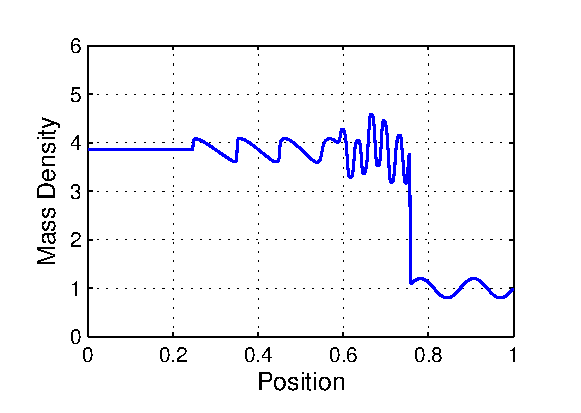
\includegraphics{ShuOsher.eps}
\caption{Shu-Osher Shocktube at t = 0.178}
\end{center}
\end{figure*}

\subsubsection{Initial Conditions}

Boundary conditions are constant around the X axis and periodic everywhere else.

The physical input parameters to the Shu-Osher test are:
\begin{itemize}
\item \tt{lambda} - Defines the wave number of the sinusoidal mass density structure
\item \tt{mach} - Defines the speed of the shockwave toward the sinusoid
\item \tt{waveAmplitude} - Defines the amplitude of the sinusoid
\end{itemize}


